\documentclass{standalone}
\usepackage{ tikz }
\usepackage{ xparse }
\usepackage{../../macros}

\begin{document}
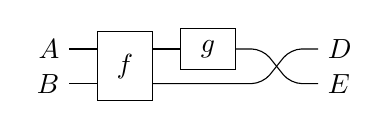
\begin{tikzpicture}[yscale=-1,x=1em,y=1.25em]
        

    \node[anchor = east] at (0,0.5){$A$};
    \node[anchor = east] at (0,1.5){$B$};

    \draw (0,0.5) -- (1,0.5);

    \draw (0,1.5) -- (1,1.5);

    \node[draw, minimum height = 2.5em, minimum width = 2em, anchor = west] at (1,1){$f$};

    \draw [rounded corners] (3,0.5) -- (4,0.5);
    \draw [rounded corners] (3,1.5) -- (7,1.5) -- (8,0.5) -- (9,0.5);
    \draw [rounded corners] (6,0.5) -- (7,0.5) -- (8,1.5) -- (9,1.5);

    \node[draw, minimum height = 1.5em, minimum width = 2em, anchor = west] at (4,0.5){$g$};

    \node[anchor = west] at (9,0.5){$D$};
    \node[anchor = west] at (9,1.5){$E$};

\end{tikzpicture}
\end{document}